\section{Pregunta N$^{\circ}$13\qquad Leon Alonzo Terrones Caccha}

\begin{frame}
    \begin{enumerate}\setcounter{enumi}{12}
        \item


              Para la función
              \begin{math}
                  f\left(t\right)=
                  \sqrt{t}
              \end{math}
              use diferencias divididas para construir el polinomio
              de Newton de grado $2$ para los puntos $t_{0}=0$,
              $t_{1}=1$ y $t_{2}=3$.
    \end{enumerate}

    \begin{solution}

        \begin{figure}[ht!]
            \centering
            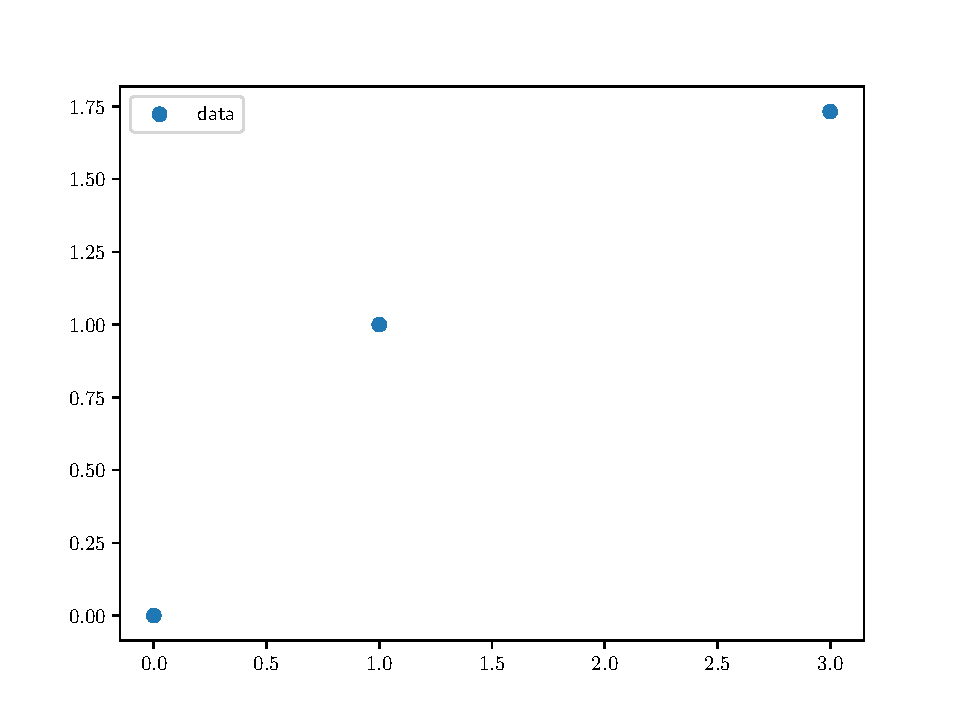
\includegraphics[width=.6\paperwidth]{p13}
        \end{figure}
    \end{solution}
\end{frame}